\section{Fundamentação Teórica}
Modulações angulares podem ser realizadas variando tanto a frequência quanto a fase de uma onda senoidal. Quando a frequência varia, tem-se uma modulação em frequência (FM) e quando a fase varia, tem-se uma modulação por fase (PM).
\par
Na modulação em frequência, a variação da frequência é dada pela derivada de $\phi(t)$, resultando na frequência instantânea mostrada na Equação \ref{eq01} \cite{proakis}:

\begin{equation}
    f_i(t) = f_c + \frac{1}{2\pi}\frac{d}{dt} \phi(t)
    \label{eq01}
\end{equation}

E a variação da frequência é expressa como:

\begin{equation}
    f_i(t) - f_c = k_f m(t) = \frac{1}{2\pi}\frac{d}{dt} \phi(t)
    \label{eq02}
\end{equation}

Onde $m(t)$ a mensagem original a ser modulada e $k_f$ é a sensibilidade da frequência, relacionando a amplitude do sinal modulador com a variação da frequência da portadora \cite{proakis}. 

Para gerar o sinal modulado, é importante entender como $\phi(t)$ é composto:

\begin{equation}
    \phi(t) = 2\pi k_f \int_{-\infty}^{t} m(\tau) \,d\tau
    \label{eq03}
\end{equation}

Ao partir da expressão geral de uma modulação angular, Equação \ref{FM-equation}, e detalhar a composição da expressão de $\phi(t)$, chega-se a uma expressão, Equação \ref{eq04},  que generaliza um sinal modulado em frequência; na qual encontram-se parâmetros como frequência da portadora e da mensagem, amplitude do sinal e uma constante $\beta_f$.

Partindo da expressão geral de uma modulação angular Equação \ref{FM-equation} e detalhando $\phi(t)$, chega-se à expressão que generaliza um sinal modulado em frequência:

\begin{equation}
    u(t) = A_ccos(2\pi f_ct + \beta_f sin(2\pi f_m t))
    \label{eq04}
\end{equation}

A constante $\beta_f$, índice de modulação, sintetiza a relação entre a sensibilidade da frequência, a amplitude $a$ da mensagem original e a frequência da mensagem. Essa relação é mostrada abaixo:

\begin{equation}
    \beta_f = \frac{k_f a}{f_m} = \frac{k_f max[|m(t)|]}{W}
    \label{eq05}
\end{equation}

Sendo $a$, o maior valor para o módulo de $m(t)$ e $W$, a largura de banda para $m(t)$. 

Para um sinal senoidal, a equação geral pode ser expressa usando a relação de Euler \cite{proakis}:

\begin{equation}
    u(t) = Re(A_c e^{j2\pi f_ct}e^{j\beta sin 2\pi f_mt})
    \label{eq06}
\end{equation}

Como $sin(2\pi f_mt)$ é periódico, é possível obter uma representação desse sinal por uma expansão por série de \textit{Fourier}, de forma que os coeficientes da série são obtidos por uma integral específica, denominada de função de \textit{Bessel} de primeira espécie de ordem $n$ \cite{proakis}.

Usando a função de Bessel de primeira espécie de ordem nn, podemos representar o sinal modulado:

\begin{equation}
    u(t) = \sum_{-\infty}^{\infty} A_c J_n (\beta) cos(2\pi(f_c + nf_m)t) 
    \label{eq07}
\end{equation}

Expressar um sinal modulado em frequência através da função de \textit{Bessel}, Equação \ref{eq07}, permite que se infira que há a presença de harmônicas, embora as amplitudes de harmônicas maiores tenham menor peso \cite{proakis}. 

\subsection{Modulação FM}
Um método para a geração de um sinal FM é utilizar um VCO (Oscilador Controlado por Voltagem), no qual a frequência é alterada em função da tensão de entrada \cite{proakis}. Quando a tensão é nula, o oscilador gera uma onda senoidal de frequência $f_c$; e conforme a tensão muda, a frequência muda de acordo com a tensão. O comportamento do VCO pode ser visualizado pela Equação \ref{eq02}, no qual quando $m(t)$ é nulo, a frequência será a $f_c$ e conforme o valor de $m(t)$ é alterado, o valor para a frequência instantânea, $f_i (t)$ também é variada. 

\subsection{Demodulação FM}
Demoduladores de sinais modulados em frequência são implementados convertendo o sinal modulado em um sinal AM (Modulado por Amplitude) \cite{proakis}, cuja amplitude varia em função da frequência instantânea do sinal modulado. Para realizar essa conversão, utiliza-se uma faixa de banda na qual a resposta em frequência possui um comportamento aproximadamente linear, de forma que a variação em frequência consiga gerar uma variação em amplitude, de forma linear, conforme a Figura \ref{fig01}.

\begin{figure}[!htb]
	\centering
	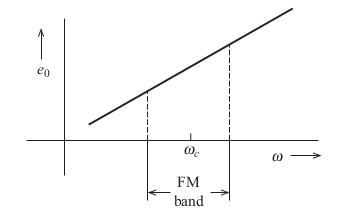
\includegraphics[width=1\linewidth]{Imagens/fig01.png}
	\caption{Resposta em frequência de um demodulador FM.}
	\label{fig01}
\end{figure}


Sendo o sinal a ser demodulado uma junção das equações \ref{FM-equation} e \ref{eq03}
\begin{equation}: 
    u(t) = A_c cos(2 \pi f_ct + 2\pi k_f \int_{-\infty}^{t} m(\tau) \,d\tau )
    \label{eq09}
\end{equation}

É possível, ao utilizar um diferenciador ideal \cite{lathi}, obter a seguinte resposta:

\begin{equation}
    u'(t) = \frac{d}{dt} 
    \Biggl\{
    Acos
    \Bigr[
    2\pi f_ct + 2\pi k_f \int_{-\infty}^{t} m(\tau) \,d\tau
    \Bigr]
    \Biggl\}
    \label{eq10}
\end{equation}

Cujo diferencial se torna:

\begin{equation}
    u'(t) = A_c \bigr[ 2\pi f_ct + k_f m(t) \bigr]
    sin \biggr[ 2\pi f_ct + 2\pi k_f \int_{-\infty}^{t} m(\tau) \,d\tau \biggr]
    \label{eq11}
\end{equation}

Dessa forma, é possível verificar na Equação \ref{eq11} o envelope $A[2\pi f_ct + k_f m(t)]$ controlando a amplitude do sinal senoidal \cite{lathi}. A Figura \ref{fig02} explicita a presença do envelope obtido pela diferenciação. 


\begin{figure}[!htb]
	\centering
	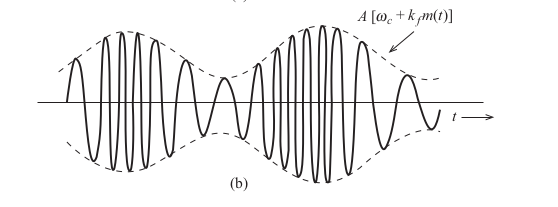
\includegraphics[width=1\linewidth]{Imagens/fig02.png}
	\caption{Saída do sinal FM em um diferenciador.}
	\label{fig02}
\end{figure}

Com a obtenção do envelope, ou seja, após a conversão do sinal FM em um AM, é possível utilizar um demodulador AM para que se obtenha a estimativa do sinal original. 